% ju 14-5-22
\section*{Einleitung}

\emph{Sonderzeichen}  wie >>\& oder \%<< müssen mit einem Backslash \verb|\& oder \%| maskiert werden, 
damit sie von LaTeX nicht als Befehle missverstanden werden.

Tabellenbuch (\textcite{bell:2021:tabellenbuchKfz} S. 281)

\emph{Website} \footnote{\url{\website}} 

\clearpage
\section*{Abbildungen}%\label{sec:Abbildungen}\index{Abbildungen}
			
	\begin{figure}[!h]
	\centering
	\subcaptionbox{Logo 1 \label{logo1}}
	{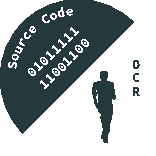
\includegraphics[width=0.35\textwidth]{images/Logo/Logo1}}
	\subcaptionbox{Logo 2 \label{logo2}}
	{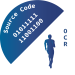
\includegraphics[width=0.35\textwidth]{images/Logo/Logo2}}
	\caption{Zwei Logos}\label{Logos}
	\end{figure}

\clearpage
\section*{Text und Abbildungen}%\label{sec:TAbbildungen}\index{Text, Abbildungen}
	%Logo in Neg, Grau, Schwarz (\autoref{fig:logoneggrauschwarz}).
	%
	\begin{figure}[!h]% hier: !hb
		\centering
		\begin{minipage}[c]{0.45\textwidth}
			Liste
			\begin{itemize} 
				\item Punkt
				\item Punkt
				\item Punkt
				\item Punkt
			\end{itemize}
		\end{minipage}
		\hfill
		\begin{minipage}[c]{0.45\textwidth}
			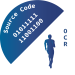
\includegraphics[width=\textwidth]{images/Logo/Logo2}%
		\end{minipage}
		%\caption{Logo in Blau}\label{fig:logoblau}%% anpassen
	\end{figure}



